\documentclass{sigchi}

% Use this command to override the default ACM copyright statement (e.g. for preprints). 
% Consult the conference website for the camera-ready copyright statement.


%% EXAMPLE BEGIN -- HOW TO OVERRIDE THE DEFAULT COPYRIGHT STRIP -- (July 22, 2013 - Paul Baumann)
% \toappear{Permission to make digital or hard copies of all or part of this work for personal or classroom use is 	granted without fee provided that copies are not made or distributed for profit or commercial advantage and that copies bear this notice and the full citation on the first page. Copyrights for components of this work owned by others than ACM must be honored. Abstracting with credit is permitted. To copy otherwise, or republish, to post on servers or to redistribute to lists, requires prior specific permission and/or a fee. Request permissions from permissions@acm.org. \\
% {\emph{CHI'14}}, April 26--May 1, 2014, Toronto, Canada. \\
% Copyright \copyright~2014 ACM ISBN/14/04...\$15.00. \\
% DOI string from ACM form confirmation}
%% EXAMPLE END -- HOW TO OVERRIDE THE DEFAULT COPYRIGHT STRIP -- (July 22, 2013 - Paul Baumann)


% Arabic page numbers for submission. 
% Remove this line to eliminate page numbers for the camera ready copy
% \pagenumbering{arabic}


% Load basic packages
\usepackage{balance}  % to better equalize the last page
\usepackage{graphics} % for EPS, load graphicx instead
\usepackage{times}    % comment if you want LaTeX's default font
\usepackage{url}      % llt: nicely formatted URLs
\usepackage{tabulary}

% llt: Define a global style for URLs, rather that the default one
\makeatletter
\def\url@leostyle{%
  \@ifundefined{selectfont}{\def\UrlFont{\sf}}{\def\UrlFont{\small\bf\ttfamily}}}
\makeatother
\urlstyle{leo}


% To make various LaTeX processors do the right thing with page size.
\def\pprw{8.5in}
\def\pprh{11in}
\special{papersize=\pprw,\pprh}
\setlength{\paperwidth}{\pprw}
\setlength{\paperheight}{\pprh}
\setlength{\pdfpagewidth}{\pprw}
\setlength{\pdfpageheight}{\pprh}

% Make sure hyperref comes last of your loaded packages, 
% to give it a fighting chance of not being over-written, 
% since its job is to redefine many LaTeX commands.
\usepackage[pdftex]{hyperref}
\hypersetup{
pdftitle={SIGCHI Conference Proceedings Format},
pdfauthor={LaTeX},
pdfkeywords={SIGCHI, proceedings, archival format},
bookmarksnumbered,
pdfstartview={FitH},
colorlinks,
citecolor=black,
filecolor=black,
linkcolor=black,
urlcolor=black,
breaklinks=true,
}

% create a shortcut to typeset table headings
\newcommand\tabhead[1]{\small\textbf{#1}}


% End of preamble. Here it comes the document.
\begin{document}

\title{Visualizing the Statewide Impact of a Revenue-Neutral Carbon Tax}

\numberofauthors{4}
\author{
  \alignauthor Justin Bare\\
    \affaddr{University of Washington}\\
    \affaddr{Seattle, WA, USA}\\
    \email{jbare@cs.washington.edu}\\
    \affaddr{}
  \alignauthor Nandita Anand\\
      \affaddr{University of Washington}\\
      \affaddr{Seattle, WA, USA}\\
      \email{nanand@uw.edu}\\
      \affaddr{}
  \alignauthor Aditya Kaul\\
      \affaddr{University of Washington}\\
      \affaddr{Seattle, WA, USA}\\
      \email{kaul10@uw.edu}\\
      \affaddr{}
  \alignauthor Zehang Richard Li\\
      \affaddr{University of Washington}\\
      \affaddr{Seattle, WA, USA}\\
      \email{lizehang@uw.edu}\\
      \affaddr{}
}

\maketitle

\begin{abstract}
We envision using online tools to introduce information into the political sphere in ways that are transparent and fair, and that hold the producers of facts accountable for the information they provide. As a prototypical example, we are developing an online calculator for a revenue-neutral carbon tax proposal in the state of Washington. The data visualization discussed here is one of the features of this tool aimed at facilitating voters' understanding of the policy and its impacts. We hope that features such as these will provide a basis of information from which democratic processes can proceed more effectively. Following the tradition of exploratory visualizations, our tool allows users to find their own insights from a large body of data using various filtering options and both broad and specific views of the data. 

\end{abstract}

\keywords{
	Exploratory visualization, Value Sensitive Design; politics
}

%\category{H.5.m.}{Information Interfaces and Presentation (e.g. HCI)}{Miscellaneous}

%See: \url{http://www.acm.org/about/class/1998/}
%for more information and the full list of ACM classifiers
%and descriptors. \newline
%\textcolor{red}{Optional section to be included in your final version, 
%but strongly encouraged. On the submission page only the classifiers’ 
%letter-number combination will need to be entered.}

\section{Introduction}
\begin{figure*}[t]
\centering
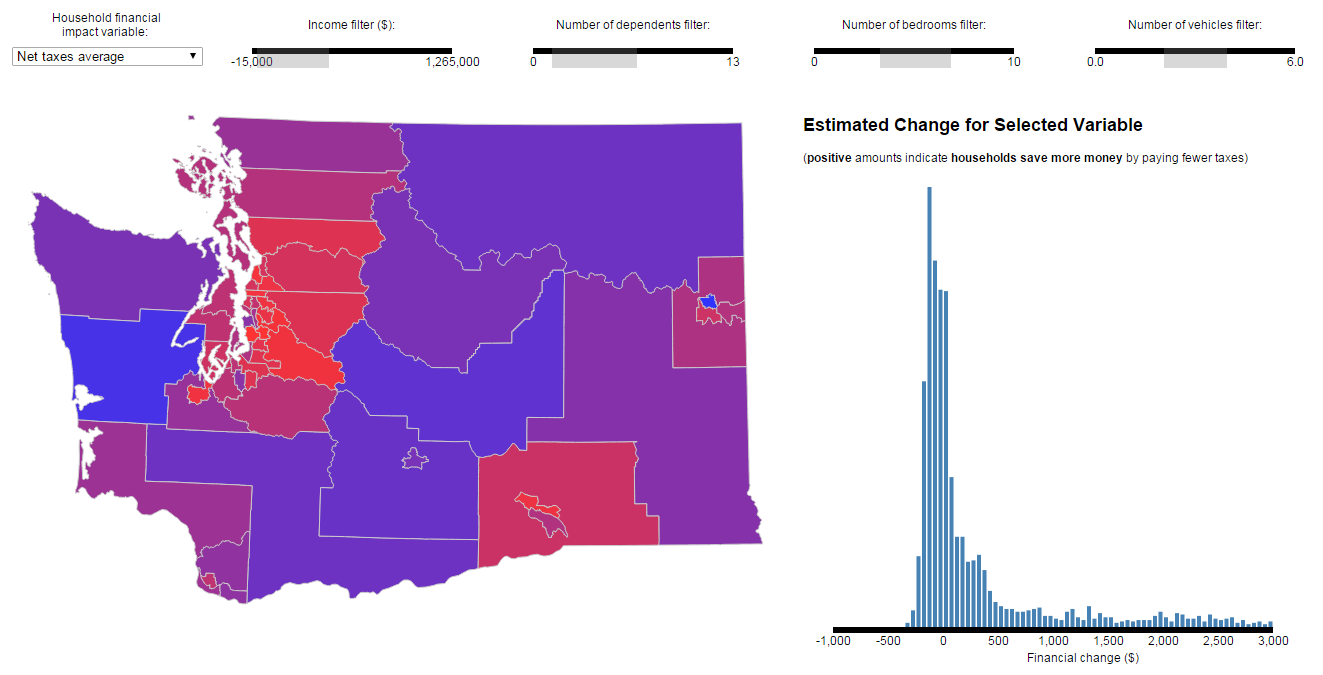
\includegraphics[width=0.9\textwidth]{summary}
\caption{The variable selector, filter brushes, map, and histogram. Filtering is being shown here with the gray brushes adjusted to custom settings by the user.}
\label{fig:summary}
\end{figure*}
Our overall goal with the carbon tax calculator project is to provide high-quality information for the debate around the Carbon Washington revenue-neutral carbon tax initiative \cite{carbonWA}, as well as a model of software development that can be replicated by others for other political issues. We aim to create a tool that supports the values that people desire from their information sources - in particular the values of transparency, fairness, and accountability. While this specific project deals with only one proposed ballot initiative, we hope that the design process and features developed will be transferable to many other political issues.

Data visualization clearly plays an important part in the pursuit of this goal because modern policies are often very complex and thus difficult for most citizens to understand fully by reading the language of the policy. Data visualization can fill this critical need by distilling complex language and calculations into relationships among visual objects that can be readily understood through graphical perception. 

To give some background on the specific policy considered here, the Carbon Washington revenue-neutral carbon tax proposal is composed of four main parts: 
\begin{enumerate}
\item reducing the state sales tax,
\item funding a tax rebate for low income households,
\item eliminating a business tax for manufacturers,
\item and instituting a tax on fossil fuels.
\end{enumerate}
“Revenue-neutral” means that the total amount that the Washington state government raises 
from taxes every year will not change significantly as a result of this policy. The revenue 
reductions (1 and 3 above) and the additional spending (2) will be balanced by the new 
revenue source of the tax on fossil fuels (4).  

This policy affects many social, economic, and environmental variables in Washington state. By creating a visualization of the statewide impact of this policy, we hope to clarify for voters the relationships among these variables so that they can make a better informed decision when voting on the ballot initiative. Also, with this information, we hope to plant the seeds for effective debate about the policy in which the tradeoffs among political values can be discussed with fewer doubts about the basic facts of the policy interrupting the discussions.

The tool discussed here will add to a previously developed tool which is the individual household carbon tax calculator for the Carbon Washington policy (see http://carbon.cs.washington.edu/). Adding this statewide impact tool is important because many people will have concerns beyond the impact the policy would have on their own household. 

\section{Related Work}
\begin{figure*}[t]
\centering
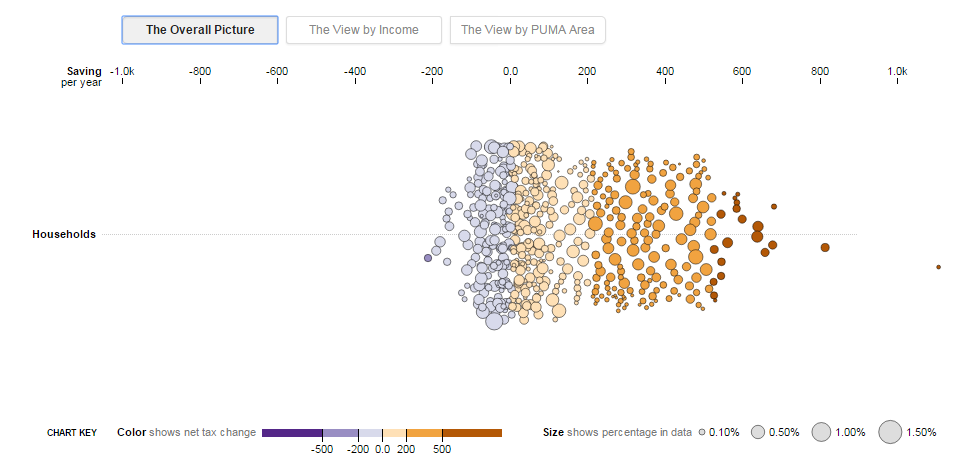
\includegraphics[width=0.9\textwidth]{bubbleOverall}
\caption{The bubble chart, show in its default view with all the households together along one axis. Vertical position has no significance in terms of information with this part of the tool. By clicking the buttons shown, the user can split the household bubble by income or Public Use Microdata Area (PUMA).  }
\label{fig:bubbleOverall}
\end{figure*}
Visualizing the impacts of the carbon tax policy is a high-dimensional problem by nature. There are several previous efforts in visually presenting similar data, both with and without geographic information. One of the most relevant visualizations is from the CoolClimate network project in Berkeley \cite{coolclimate} where an interactive map of carbon footprints at zipcode level is provided for all the states in US where the measurement for each zipcode is shown by a different color. Similar visualizations have been seen elsewhere too \cite{almanac, powerplant}, where icons are used effectively to let users observe more detail upon zooming in. As for the non-geographic aspects, it is typically difficult to present efficient visualization of high dimensional data \cite{seo2005rank}. There have been many successes, however, in visualizing selected dimensions of the data for better story-telling. For example, \cite{nytimes} shows interesting ways to segment high dimensional data using a bubble graph or Sankey diagram, which also inspires our work on non-geographic data. Connectivity and coherency between visualizations are also of great importance. \cite{nytimes-map} shows correspondence between geographic and non-geographic representations. In addition, narratives and animation techniques are also a natural supplement to enhancing the effectiveness of visualizations for similar data \cite{jheer-animation, jheer-narrative}. 


\section{Methods}

All of our code was written in HTML, CSS, and Javascript and we used the D3 Javascript library to accomplish our visualization goals as described in the following sections.

\subsection{Update Design Pattern}
Our general framework for updating the map, histogram, and bubble chart modules was designed so as to reduce the amount of computation required in order to speed up execution time to provide a better, smoother experience for users. To do this, we only read the raw data once during the website initialization. From then on, we accomplished view updates by passing around an update object which specifies the parameters necessary to accomplish the appropriate data filtering in response to mouse click events and drag events. 

\subsection{Map}
To create the geographical boundaries in our map visualization, we obtained the shapefile of the Public Use Microdata Areas (PUMAs, which are the geographic location variables from our dataset \cite{pums}), filtered this to a dataset containing only Washington state PUMAs, and then translated this into a TopoJSON file for use with D3. We used the Albers projection to transform the sphere of the globe into two dimensions to display the map because this is the standard projection used for the United States that preserves area. We enabled zooming on the map via mouse click by computing the centroid of the PUMA that the user clicks and using these coordinates to guide the view to focus on a smaller region of the state. 

\subsection{Histogram}
The histogram was implemented using D3's histogram functionalities to bin the data appropriately.

\subsection{Bubble}
A goal of our visualization is to show the relationship between both geographic areas and income groups. The map and bar chart visualization provides detailed insight into each area with customized data filtering, but it is difficult to compare two dimensions of the data at the same time. For example, to answer questions such as which income group is affected most in an area, a user needs to change the filter constantly and explore the changes on the map. Such questions, however, would be of interest to voters since it reflects the more general question of ``from where do my tax savings come'' or ``to where does my increased tax money go'' since this carbon tax policy can be thought of as just a shift in the tax system, with tax burdens and benefits being redistributed slightly. Our initial plan was to show the flow of the tax change between typical household types.  However, as we explored the data it became less clear what a ``typical household'' meant in our context. Considering the potentially high dimensionality of household characteristics, and the limitation of data availability, the final implementation is carried out with only the interaction between area and income group, as they are the two most important variables in our analysis.  Also instead of showing the flow of changes, we represent households in the same income group in each area as a bubble and arrange them horizontally by the measurement of interest for a cleaner visualization. The color scheme and graph representation is inspired by the New York Times visualization \cite{nytimes}. We extended the original visualization to make it more flexible in terms of interactivity.

\subsection{Interactivity}
There are five essential components of our visualization, namely the map, histogram, bubble chart, drop down list and filters.
The drop down list gives the user the option to choose different variables that impact the household finance.
The map represents the different PUMAs in the state of Washington. Since some of the PUMAs are extremely small in area, we implemented the zoom feature to enable the users to zoom into any area of their choice. On hovering over any of the areas a tooltip is enabled which gives the user information about the region. These details include the name of the PUMA, the PUMA code number and the average financial impact for the variable that is selected.
The data for the histogram changes depending on the area selected in the map. Similar to the map, on hovering over the histogram the user gets additional information via the tool tip. It is important to note here that the histogram represents the value of a particular variable in the drop down. On selecting a different variable in the drop down we get a different histogram altogether.
To further enable the users to control the data they see, we have provided filters that let the users limit the data used in the map and histogram. These were built using D3's brush features. 
The bubble chart is divided into three sections such that it gives us the overall information as to how a certain variable, which we selected from the drop down, is affected over the entire state. We can get more intricate details by expanding the bubble chart on basis of the income or the PUMA area code. Similar to the map and the histogram the user can get some additional information by simply hovering the mouse over the bubbles. 

\subsection{Data}
The main source of data used for our visualization is from the Public Use Microdata Sample (PUMS) collected by the American Community Survey. We use the 2009-2013 5-year PUMS household data for the state of Washington \cite{pums} . The original dataset consists of records for 156,867 households in the state, including many variables such as the household gross income, household type, number of dependents, etc. In particular, the dataset contains geographic locations for each household sample in the form of Public Use Microdata Areas (PUMAs), which are special non-overlapping partitions of states so that each area contains no fewer than 100,000 people each. The location information for each household makes our geographic visualization of carbon tax impact possible. For the purpose of the carbon tax calculation, the key variables extracted from the dataset are gross household income, number of dependents, marital status, home heating fuel type, and number of bedrooms. We thus use only the 89,643 households which have no missing data among these variables. 

To have useful data for our purposes, we had to compute new variables from the survey and statistical data according to the mathematical calculations specified in the proposed carbon tax policy. These new variables included household tax savings from the sales tax reduction and working families rebate, as well as additional tax payments for fossil fuel intensive activities, in particular vehicle fuel consumption, air travel, and home energy consumption. The sales tax savings for each household are estimated from the household income \cite{salesTax}. The working families rebate is estimated using income, number of dependents, and marital status \cite{eitc}. The additional gasoline tax amount is computed for each income group from the national average gasoline consumption reported in the Consumer Expenditure Survey \cite{ces}. Unfortunately we had no available data to compute the additional air travel taxes. 

The most technically difficult variable to compute was home energy consumption. We used custom data created by Carbon Washington that lists the utilities in each zipcode and the percentage of electricity produced from fossil fuels by each utility in the state. To use this with the PUMS data, we computed the utilities in each PUMA using data on the correspondence between zipcodes and PUMAs \cite{missouri}. From the list of utilities for each PUMA, we computed the best, worst, and average percentages of electricity from fossil fuels. Finally, we used these values along with the number of bedrooms (as an approximation of house size) and house heating fuel type to compute the expected best, worst, and average possible additional home energy taxes for each household in the PUMS data. 


\section{Results}
The results of our design are shown in Figures \ref{fig:summary}, \ref{fig:bubbleOverall}, \ref{fig:bubbleIncome}, and \ref{fig:mapTooltip}. 

Figure \ref{fig:summary} shows the main view. Using the filters and location information from the map, users can fairly easily focus in on particular households from the survey that might be similar to their own household. Including the map was very important because we want our users to be engaged with the data. Being able to see the effects of the policy in their actual location in the state makes the data exploration a much more personal process. Also, the map reveals interesting features of the underlying data. For example, selecting ``Electricity taxes best'' reveals a very odd map that is mostly blue with three red areas. This indicates that only these three areas out of all the areas in the state have no access to a utility provider that does not use mostly fossil fuels. 

As shown in Figure \ref{fig:bubbleOverall}, this bubble chart representation allows users to easily expand the bubble chart by either income group (see Figure \ref{fig:bubbleIncome}) or area and compare the distribution of households in each category. For example, by showing the net tax savings by income group, users might find from the curved trend that income groups at both the lower and higher ends of the spectrum on average enjoy higher savings than the middle-income households. The area effect within each income group could also be examined by comparing the bubbles in each expanded row. Thus it provides easier visualization of general trends that are otherwise difficult to observe from the map. Also the sample size in each bubble is represented by size, so smaller areas with dense population could be compared more easily. We explored different ways to jitter the bubbles so they are non-overlapping. The final version uses positions pre-calculated by an iterative algorithm of our own implementation. For some of the measurements, the position of the bubbles are still partially overlapped, mostly due to the low variability in those measurements.  

\begin{figure}
\centering
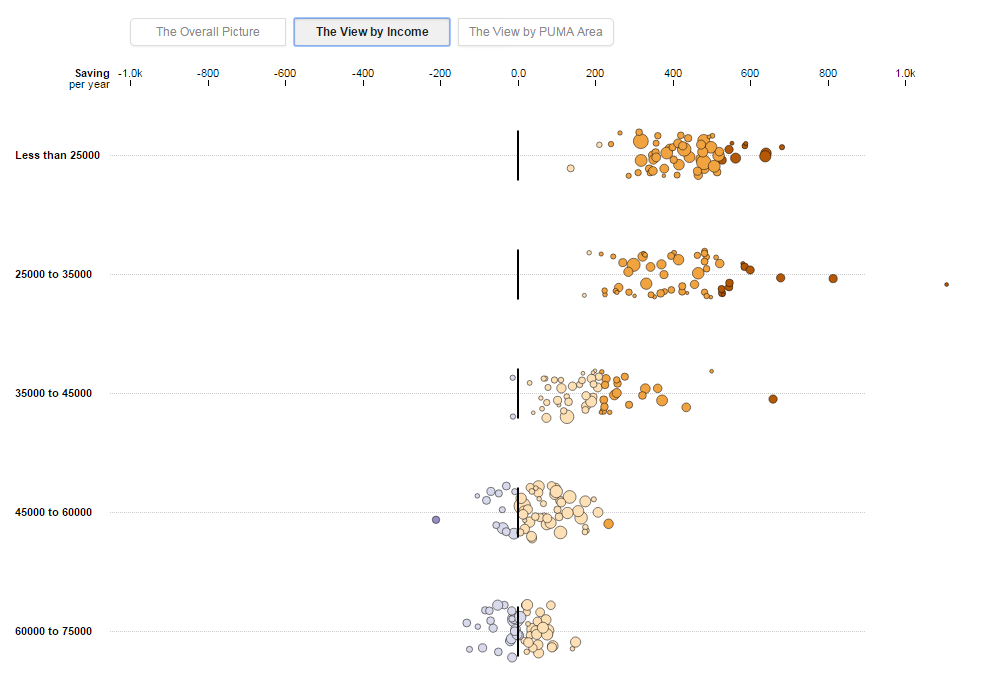
\includegraphics[width=0.45\textwidth]{bubbleIncome}
\caption{The interaction of splitting the bubble chart by income. }
\label{fig:bubbleIncome}
\end{figure}

Finally, Figure \ref{fig:mapTooltip} shows an important interaction feature that is present in the map, histogram, and bubble chart, which is the tooltip. We thought this was essential since it is difficult to read exact values for many of the data encodings used in the visualizations. Also, the tooltips provide interesting metadata that may keep users more engaged. For example, the map tooltip shows names of counties or cities encompassed by the PUMA boundary. Also, the histogram tooltip shows the number of households in each bin, which could be neat if the user has a very rare household profile and can filter the data down to a few samples that are similar. 

\begin{figure}
\centering
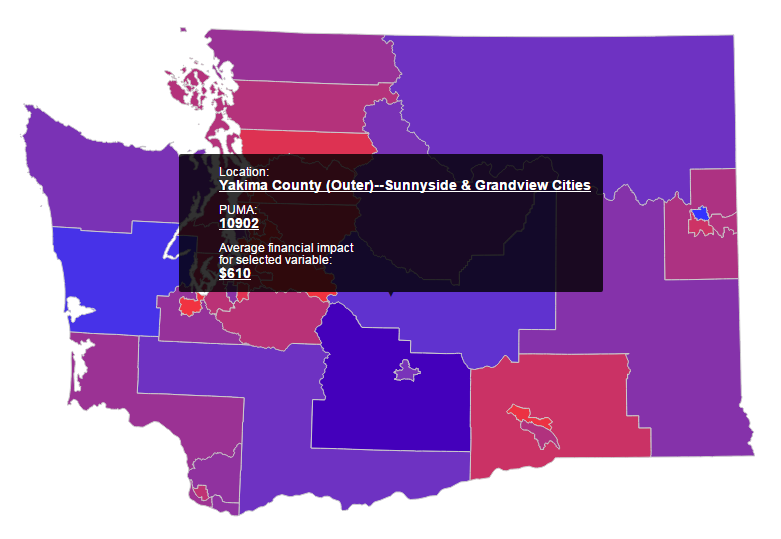
\includegraphics[width=0.45\textwidth]{mapTooltip}
\caption{The tooltip appears to offer more information when the user hovers over a map region. }
\label{fig:mapTooltip}
\end{figure}

\section{Discussion}
Our work shows that the impacts of public policies can be made accessible to more people than just the experts. Through exploratory data visualization techniques, visualizations can be created to allow average voters to roll up and drill down through the data using different graphical encodings in order to better understand the high-dimensional possible impacts of policies. 

One of the limitations of the current implementation is that the bubble chart is not linked to the data filtering of the map. Currently the aggregation of measurements and the layout of the bubbles are pre-computed separately. More efficient ways to automatically aggregate from the user-selected data and calculate positions remain to be explored. By allowing bubble position to be determined dynamically more interactions could also be made possible, such as the merging and splitting of the bubbles at customized dimensions. 

One of the reviews we got for the current visualization was the lack of intuitiveness in the filters. In the future, we would like to work on improving the filters and make them more intuitive. We would also like to improve the data encodings used. As an example, we would like to improve the colors and add legends to make the visualization both aesthetically pleasing and more informative. In order to allow for an effective and efficient user interaction, we would also like to work more on implementing helpful transitions not only in a particular module of the visualization but also between modules.


\section{Future Work}
A major setback we faced in the current visualization involved lack of comprehensive data sets. We used data from multiple sources and also faced the problem of missing data. As a part of future work we would attempt to get more comprehensive and complete datasets, or commission our own surveys to gather appropriate data for the variables we wish to represent. Another option would be to allow users of the original individual calculator tool (http://carbon.cs.washington.edu/) to submit their exact data to be added to the visualization we have created here, thus forming our own, more accurate dataset. 

One very helpful piece of feedback we received was that the visualization could benefit from some kind of guided tutorial when the page loads in order to familiarize users with the controls and the meanings of the data representations, especially since it is currently difficult for new users to figure out if positive dollar amounts are good or bad (``does that mean I'm paying more taxes or saving more money?''). We had initially thought about using narrative in our visualization, but we could not think of a way to fit it in logically to our exploratory system, but this tutorial would be a feature for which effective narrative design would be crucial. 

Finally, we consider user input, comments, and critique as an important component of developing a good and useful visualization system/application. Thus, we would like to eventually complete a formal user study and evaluation, which we did not have time to do in this course. This would involve running lab tests with users completing various tasks using the visualization we've developed. Also, objective measurements of performance, such as execution time on user-initiated mouse events, would be important factors to analyze to assess the effectiveness of our visualization. 


\section{Acknowledgments}

This material is based upon work supported by the National Science Foundation
Graduate Research Fellowship Program under Grant No. DGE-1256082.

% Balancing columns in a ref list is a bit of a pain because you
% either use a hack like flushend or balance, or manually insert
% a column break.  http://www.tex.ac.uk/cgi-bin/texfaq2html?label=balance
% multicols doesn't work because we're already in two-column mode,
% and flushend isn't awesome, so I choose balance.  See this
% for more info: http://cs.brown.edu/system/software/latex/doc/balance.pdf
%
% Note that in a perfect world balance wants to be in the first
% column of the last page.
%
% If balance doesn't work for you, you can remove that and
% hard-code a column break into the bbl file right before you
% submit:
%
% http://stackoverflow.com/questions/2149854/how-to-manually-equalize-columns-
% in-an-ieee-paper-if-using-bibtex
%
% Or, just remove \balance and give up on balancing the last page.
%
\balance

% REFERENCES FORMAT
% References must be the same font size as other body text.
\bibliographystyle{acm-sigchi}
\bibliography{sample}
\end{document}
